\documentclass[11pt]{article}
\usepackage[utf8]{inputenc}
\usepackage[shortlabels]{enumitem}
\usepackage{amsmath}
\usepackage{amssymb}
\usepackage{amsthm}
\usepackage{xcolor}
\usepackage{graphicx}
\usepackage{blkarray}

\usepackage{hyperref}
\hypersetup{
    colorlinks=true,
    linkcolor=blue,
    filecolor=magenta,      
    urlcolor=cyan,
}


% setting page format
\topmargin -.5in
\textheight 9in
\oddsidemargin -.25in
\evensidemargin -.25in
\textwidth 7in
\setlength{\parindent}{0 in}
\setlength{\parskip}{0.1 in}

% setting new environments
\newtheorem*{theorem}{Theorem}
\newtheorem*{lemma}{Lemma}
\newtheorem*{corollary}{Corollary}

\theoremstyle{definition}
\newtheorem*{definition}{Definition}
\newtheorem*{example}{Example}
\newtheorem*{problem}{Problem}
\newtheorem*{question}{Question}

\theoremstyle{remark}
\newtheorem*{remark}{Remark}

\newenvironment{solution}[1][Solution]{\textbf{#1:} \par}{\ $\blacksquare$}

\newenvironment{newnotion}[1]{\textbf{#1.}}

\newenvironment{caution}{$\bigstar\bigstar\bigstar$\textbf{Caution.}}

%\newenvironment{proof}[1][Proof]{\textbf{#1:} \par}{\ \rule{0.5em}{0.5em}}
%\newenvironment{problem}[1]{\textbf{#1:} }

% define new commands
\renewcommand{\hat}{\widehat}
\renewcommand{\tilde}{\widetilde}

\newcommand{\numpy}{{\tt numpy}}    % tt font for numpy
\newcommand{\dom}[1]{\mathbf dom #1}
\newcommand{\tr}{\mathbf{tr}}
\newcommand{\sgn}{\text{sgn}}
\newcommand{\spacevert}{\;\vert\;}
\newcommand{\ie}{i.e.}
\newcommand{\eg}{e.g.}

\newcommand{\N}{\mathbb{N}}
\newcommand{\E}{\mathbb{{E}}}
\newcommand{\Q}{\mathbb{Q}}
\newcommand{\R}{\mathbb{R}}
\newcommand{\C}{\mathbb{C}}
\newcommand{\Z}{\mathbb{Z}}
\newcommand{\mS}{\mathbb{S}}

% for probability
\newcommand{\Exp}{\mathbf{E}}
\newcommand{\Var}{\mathbf{Var}}
\newcommand{\Prob}{\mathbf{P}}
\newcommand{\card}{\mathbf{card}}
\newcommand{\cov}{\mathbf{cov}}
\newcommand{\corr}{\mathbf{corr}}
\newcommand{\1}{\mathbf{1}}


% for optimizations
\newcommand{\subto}{\text{s.t.}}

% for norms
\newcommand{\norm}[1]{\left\Vert #1 \right\Vert}
\newcommand{\abs}[1]{\left\vert #1 \right\vert}

\begin{document}
% ========== Edit your name here
\title{MATH 2901 Basic Probability Lecture Notes 9}
\author{Instructor: Richard Kleeman}
\date{}
\maketitle

%\medskip

% ========== Contents begin here ==============
## Random walk
### Basic defitions

One of the simplest random processes is so-called ``simple 
random walk". 

<div class="theorem-block"><p><b>Definition.<b> 
Let $\{X_k\}_{k=1}^\infty$ be a sequence of i.i.d. discrete random variables with finite outcomes. For each positive integer $n$, we let $S_n$ denote the sum $X_1 +X_2 + \cdots + X_n$. The sequence $\{S_n\}_{n=1}^\infty$ is called a **random walk**.
</p></div>

<div class="remark-block"><p><b>Remark.<b> 
If the common range of the $X_k$’s is $\mathbb{R}^m$, then we say that $\{S_n\}$ is a random walk in $\mathbb{R}^m$.
</p></div>

<div class="remark-block"><p><b>Remark.<b> 
Sometimes we set $S_0 = a$ for some number $a$ as the **start value** of the random walk. This is common in the gambling analysis.
</p></div>

<div class="theorem-block"><p><b>Lemma.<b> 
The simple random walk has the Markov property ; that is
$$\begin{equation}
    \mathbf{P}\left(S_{m+n}=j | S_{0}, S_{1}, \ldots, S_{m}\right)=\mathbf{P}\left(S_{m+n}=j | S_{m}\right), \quad n \geq 0.
\end{equation}$$
</p></div>

\begin{proof}
If one knows the value of $S_m$ , then the distribution of $S_{m+n}$ depends only on the jumps $X_{m+ 1} ,\dots, \\ X_{m+n}$, and cannot depend on further information concerning the values of $S_0, S_1, \dots , S_{m-1}$.
\end{proof}

The random walk has two main applications: gambling analysis and investment decision making. For example, in the gambling, we gamble at each step, $S_i$ is the total stack we have at step $i$, and we are interested in when there will be a **return** or \text{equalization}, i.e., what is the probability that $S_0 = a = S_n$.

<div class="remark-block"><p><b>Example.<b> [Random walks on the real line]
We shall first consider the simplest non-trivial case of a random walk in $\mathbb{R}^1$, namely the case where the common distribution function of the random variables $X_n$ is given by
$$$$$$$$\begin{equation}
    \label{eq:9.1}
    \tag{9-1}
    f_{X}(x)=\left\{\begin{array}{ll}{1 / 2,} & {\text { if } x=\pm 1} \\ {0,} & {\text { otherwise }}\end{array}\right.
\end{equation}$$$$$$$$
We note that in this situation, all paths of length $n$ have the same probability, namely $2^{-n}$.

We can plot the random walk in the plane, where the horizontal axis represents time and the vertical axis represents the value of $S_n$. Given a sequence $\{S_n\}$ of partial sums, we first plot the points $(n, S_n)$, and then for each $k < n$, we connect $(k, S_k)$ and $(k + 1, S_{k+1})$ with a straight line segment. The **length** of a path is just the difference in the time values of the beginning and ending points on the path. This can be visualized in Figure \ref{fig:9.1}.

\begin{figure}[!htb]
    \centering
    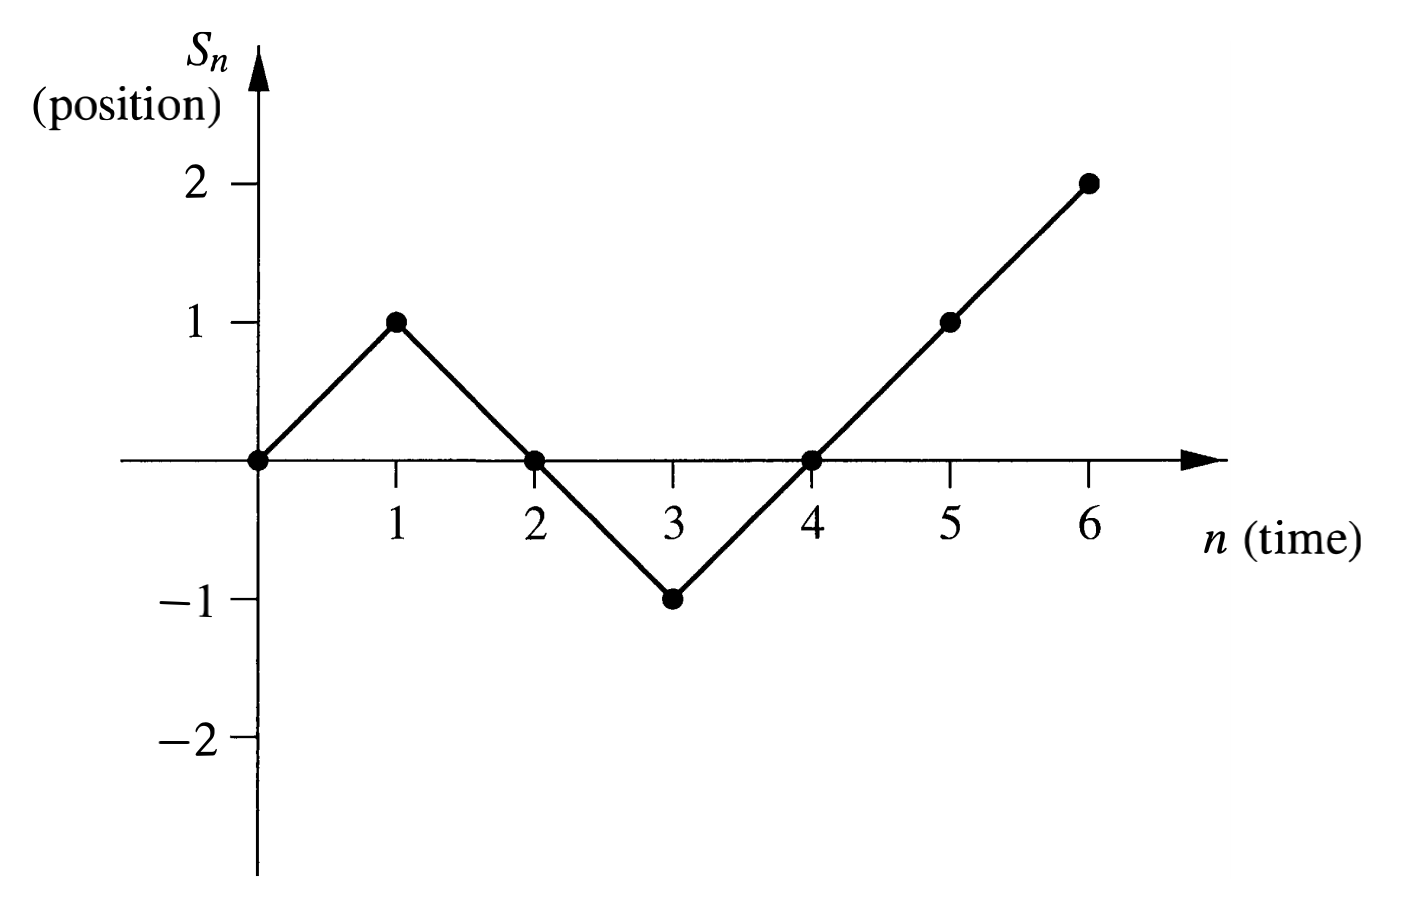
\includegraphics[scale=0.3]{plots/random_walk.png}
    \caption{A random walk $S_n$.}
    \label{fig:9.1}
\end{figure}
</p></div>



### Returns and First Returns
This subsection studies the random walk in $\mathbb{R}^1$. The p.m.f. of $X_i$ is given by \eqref{eq:9.1}.

We say that an **equalization** has occurred, or there is a **return** to the origin at time $n$, if $S_n = 0$. Note that the returns are possible **only after even number of steps**. To calculate
the probability of an equalization at time $2m$, **we need only count the number of paths of length $2m$ which begin and end at the origin**. The number of such paths is clearly
$$\begin{equation}
    \binom{2m}{m} = \frac{(2m)!}{m! m!}.
\end{equation}$$
Since each path has probability $2^{-2m}$, we have the following theorem.
<div class="theorem-block"><p><b>Theorem.<b> 
The probability of a return to the origin at time $2m$ is given by
$$\begin{equation}
    u_{2 m}= \binom{2m}{m} 2^{-2 m}.
\end{equation}$$
The probability of a return to the origin at an odd time is 0.
</p></div>

A random walk is said to have a **first return** to the origin at time $2m$ if $m > 0$, and $S_{2k} = 0$ for all $k < m$. We define $f_{2m}$ to be the probability of this event. (We also define $f_0 = 0$.) One can think
of the expression $f_{2m}2^{2m}$ as the number of paths of length $2m$ between the points $(0, 0)$ and $(2m, 0)$ that do not touch the horizontal axis except at the endpoints. We have the following theorem.
<div class="theorem-block"><p><b>Theorem.<b> 
For $n \geq 1$, the probabilities $\{u_{2k}\}$ and $\{f_{2k}\}$ are related by the equation
$$\begin{equation}
    u_{2 n}=f_{0} u_{2 n}+f_{2} u_{2 n-2}+\cdots+f_{2 n} u_{0},
\end{equation}$$
where $f_0 = 0$ and $u_0 = 1$ as convention.
</p></div>

\begin{proof}
There are $u_{2n}2^{2n}$ paths of length $2n$ which have endpoints $(0, 0)$ and $(2n, 0)$. The collection of such paths can be partitioned into $n$ sets, depending upon the time of the first return to the origin. A path in this collection which has a first return to the origin at time $2k$ consists of an initial segment from $(0, 0)$ to $(2k, 0)$, in which no interior points are on the horizontal axis, and a terminal segment from $(2k, 0)$
to $(2n, 0)$, with no further restrictions on this segment. Thus, the number of paths in the collection which have a first return to the origin at time $2k$ is given by
$$\begin{equation}
    f_{2 k} 2^{2 k} u_{2 n-2 k} 2^{2 n-2 k}=f_{2 k} u_{2 n-2 k} 2^{2 n}.
\end{equation}$$
If we sum over $k$, we obtain the equation
$$\begin{equation}
    u_{2 n} 2^{2 n}=f_{0} u_{2 n} 2^{2 n}+f_{2} u_{2 n-2} 2^{2 n}+\cdots+f_{2 n} u_{0} 2^{2 n}
\end{equation}$$
Dividing both sides of this equation by $2^{2n}$ completes the proof.
\end{proof}

Using the generating functions, we have following theorem.
<div class="theorem-block"><p><b>Theorem.<b> 
For $m \geq 1$, the probability of a first return to the origin at time
$2m$ is given by
$$\begin{equation}
    f_{2 m}=\frac{u_{2 m}}{2 m-1}=\frac{\binom{2m}{m}}{(2 m-1) 2^{2 m}}.
\end{equation}$$
</p></div>

\begin{proof}
We begin by defining the generating functions
$$\begin{equation}
    U(x)=\sum_{m=0}^{\infty} u_{2 m} x^{m}
\end{equation}$$
and 
$$\begin{equation}
    F(x)=\sum_{m=0}^{\infty} f_{2 m} x^{m}.
\end{equation}$$
Note that two sequences converge when $\left\vert x \right\vert<1$. The preceding theorem says that 
$$\begin{equation}
    U(x)=1+U(x) F(x).
\end{equation}$$
(The presence of the $1$ on the right-hand side is due to the fact that $u_0$ is defined to be $1$, but the last theorem only holds for $m \geq 1$.) We can solve the above equation for $F(x)$, obtaining
$$\begin{equation}
    F(x)=\frac{U(x)-1}{U(x)}.
\end{equation}$$
Now, if we can find a closed-form expression for the function $U(x)$, we will also have a closed-form expression for $F(x)$. From the first theorem in this notes, we have
$$\begin{equation}
    U(x)=\sum_{m=0}^{\infty}\binom{2m}{m} 2^{-2 m} x^{m} = \sum_{m=0}^\infty \binom{2m}{m} \left( \frac{x}{4} \right)^m.
\end{equation}$$
From series expansion, we find that 
$$\begin{equation}
    \frac{1}{\sqrt{1-4 x}}=\sum_{m=0}^{\infty}\left(\begin{array}{c}{2 m} \\ {m}\end{array}\right) x^{m}.
\end{equation}$$
Therefore, we have 
$$\begin{equation}
    U(x)=\frac{1}{\sqrt{1-x}}, \quad F(x) = \frac{U(x)-1}{U(x)} = 1-\sqrt{1-x}.
\end{equation}$$
Although it is possible to compute the value of f2m using the Binomial Theorem, it is easier to note that $F'(x) = U(x)/2$, so that the coefficients $f_{2m}$ can be found by integrating the series for $U(x)$. We obtain, for $m \geq 1$, 
$$\begin{equation}
    f_{2 m}=\frac{u_{2 m-2}}{2 m} = \frac{\binom{2m-2}{m-1}}{m 2^{2 m-1}} = \frac{\binom{2m}{m}}{(2 m-1) 2^{2 m}} = \frac{u_{2m}}{2m-1},
\end{equation}$$
since
$$\begin{equation}
    \binom{2m-2}{m-1} = \frac{m}{2(2 m-1)}\binom{2m}{m}.
\end{equation}$$
This completes the proof of the theorem.
\end{proof}

### Probability of Eventual Return
In the symmetric random walk process in $R^m$, we first examine this question in the case that $m = 1$, and then we consider the general case.

We should be careful when dealing with eventual return since the sample space seems to be the set of all walks of infinite length, and this set is non-denumerable. To avoid difficulties, we will define $w_n$ to be the probability that a first return has occurred no later than time $n$. Thus,
$w_n$ concerns the sample space of all walks of length $n$, which is a finite set. Then it is reasonable to define 
$$\begin{equation}
    w_{*}=\lim _{n \rightarrow \infty} w_{n}.
\end{equation}$$
This limit clearly exists and is at most one, since the sequence $\{w_n\}_{n=1}^\infty$ is an increasing sequence, and all of its terms are at most 1. In terms of the $f_n$ probabilities, we see that
$$\begin{equation}
    w_{2 n}=\sum_{i=1}^{n} f_{2 i}.
\end{equation}$$
Thus 
$$\begin{equation}
    w_{*}=\sum_{i=1}^{\infty} f_{2 i}.
\end{equation}$$
In previous proof we introduced the the generating function
$$\begin{equation}
    F(x)=\sum_{m=0}^{\infty} f_{2 m} x^{m} = 1-\sqrt{1-x}.
\end{equation}$$
which is convergent for $\left\vert x \right\vert < 1$. In fact, it also converges for $x = \pm 1$. Hence we see that 
$$\begin{equation}
    w_{*}=F(1)=1.
\end{equation}$$
Thus, with probability one, the particle returns to the origin in $\mathbb{R}^1$ random walk.

Now we consider the eventual return in $\mathbb{R}^m$. We define $f_{2 n}^{(m)}$ to be the probability that the first return to the origin in $\mathbb{R}^m$ occurs at time $2n$. The quantity $u_{2 n}^{(m)}$ is defined in a similar manner. From the preceding theorem, we have 
$$\begin{equation}
    u_{2 n}^{(m)}=f_{0}^{(m)} u_{2 n}^{(m)}+f_{2}^{(m)} u_{2 n-2}^{(m)}+\cdots+f_{2 n}^{(m)} u_{0}^{(m)}.
\end{equation}$$
We continue to generalize previous work by defining
$$\begin{equation}
    U^{(m)}(x)=\sum_{n=0}^{\infty} u_{2 n}^{(m)} x^{n}, \quad F^{(m)}(x)=\sum_{n=0}^{\infty} f_{2 n}^{(m)} x^{n}.
\end{equation}$$
Then we see that 
$$\begin{equation}
    U^{(m)}(x)=1+U^{(m)}(x) F^{(m)}(x).
\end{equation}$$
These functions will always converge in the interval $(1, 1)$. In fact, since 
$$\begin{equation}
    w_{*}^{(m)}=\sum_{n=0}^{\infty} f_{2 n}^{(m)} \leq 1
\end{equation}$$
for all $m$, the series for $F^{(m)}(x)$ converges at $x = 1$ as well, and $F^{(m)}(x)$ is left continuous at $x = 1$, i.e.,
$$\begin{equation}
    \lim _{x \uparrow 1} F^{(m)}(x)=F^{(m)}(1).
\end{equation}$$
Thus, we have
$$$$$$$$\begin{equation}
    \label{eq:9.2}
    \tag{9-2}
    w_{*}^{(m)}=\lim _{x \uparrow 1} F^{(m)}(x)=\lim _{x \uparrow 1} \frac{U^{(m)}(x)-1}{U^{(m)}(x)},
\end{equation}$$$$$$$$
so to determine $w_{*}^{(m)}$, , it suffices to determine 
$$\begin{equation}
    \lim _{x \uparrow 1} U^{(m)}(x).
\end{equation}$$
We let $u^{(m)}$ denote this limit. Then we have 
$$$$$$$$\begin{equation}
    \label{eq:9.3}
    \tag{9-3}
    u^{(m)}=\sum_{n=0}^{\infty} u_{2 n}^{(m)}.
\end{equation}$$$$$$$$

In $\mathbb{R}^2$ random walk, we have
$$\begin{equation}
    u_{2 n}^{(2)}=\frac{1}{4^{2 n}} \binom{2n}{n}^2. 
\end{equation}$$
Using Stirling’s Formula
$$$$$$$$\begin{equation}
    \label{eq:Stirling}
    \tag{Stirling}
    n! \sim n^n e^{-n} \sqrt{2\pi n} \quad \text{for  $n$  large.}
\end{equation}$$$$$$$$
we have
$$\begin{equation}
    \binom{2n}{n} \sim \frac{2^{2 n}}{\sqrt{\pi n}} \quad \mathbb{R}ightarrow \quad 
    u_{2 n}^{(2)} \sim \frac{1}{\pi n}.
\end{equation}$$
From this it follows easily that 
$$\begin{equation}
    \sum_{n=0}^{\infty} u_{2 n}^{(2)}
\end{equation}$$
diverges, so $w_{*}^{(2)}=1$, i.e., in $\mathbb{R}^2$, the probability of an eventual return is 1.

In $\mathbb{R}^3$, we have 
$$\begin{equation}
    u_{2 n}^{(3)}=\frac{1}{2^{2 n}}\binom{2n}{n} \sum_{j, k}\left(\frac{1}{3^{n}} \frac{n !}{j ! k !(n-j-k) !}\right)^{2}, 
\end{equation}$$
Note that $\sum_{n=0}^{\infty} u_{2 n}^{(3)}$ converges, so $w_{*}^{(3)}$ is strictly less than one. This means that in $\mathbb{R}^3$, the probability of an eventual return to the origin is strictly less than one.


## Gambler’s Ruin
In this section, we remove the assumption that the random walk is symmetric. Instead, we assume that $p$ and $q$ are non-negative real numbers with $p + q = 1$, and that the common distribution function of the jumps of the random walk is
$$\begin{equation}
    f_{X}(x)=\left\{\begin{array}{ll}{p,} & {\text { if } x=1} \\ {q,} & {\text { if } x=-1}\end{array}\right.
\end{equation}$$

\begin{newnotion}{Problem formulation}
A gambler starts with a ``stake" of size $s$. She plays until her capital reaches the value $M$ or the value $0$. In the language of Markov chains, these two values correspond to absorbing states. We are interested in studying the probability of occurrence of each of these two outcomes.
\end{newnotion}
We begin by defining $S_k$ to be the probability that the gambler’s stake reaches 0, i.e., she is ruined, before it reaches $M$, given that the initial stake is $k$. We note that $S_0 = 1$ and $S_M = 0$. The **fundamental relationship** among the $S_k$’s is the following:
$$\begin{equation}
    S_{k}= p S_{k+1} + q S_{k-1},
\end{equation}$$
where $1 \leq k \leq M-1$. This holds because if her stake equals $k$, and she plays one game, then her stake becomes $k + 1$ with probability $p$ and $k-1$ with probability $q$. Since $p+q = 1$, we can rewrite the equation as 
$$\begin{equation}
    p\left(S_{k+1}-S_{k}\right)=q\left(S_{k}-S_{k-1}\right) \quad \text{ or }  \quad 
    S_{k+1}-S_{k}=\frac{q}{p}\left(S_{k}-S_{k-1}\right).
\end{equation}$$
From this equation, it is easy to see that
$$\begin{equation}
    S_{k+1}-S_{k}=\left(\frac{q}{p}\right)^{k}\left(S_{1}-S_{0}\right). 
\end{equation}$$
We now use telescoping sums to obtain an equation in which the only unknown is $S_1$.
$$\begin{equation}
    \begin{split}
        -1 &= S_M - S_0 = \sum_{k=0}^{M-1}\left(S_{k+1}-S_{k}\right) \\  
        &= \sum_{k=0}^{M-1}\left(\frac{q}{p}\right)^{k}\left(S_{1}-S_{0}\right) = \left(S_{1}-S_{0}\right) \sum_{k=0}^{M-1}\left(\frac{q}{p}\right)^{k}.
    \end{split}
\end{equation}$$
Then we can solve for $S_j$, $1\leq j \leq M$:
$$\begin{equation}
    S_{j}=1-\frac{(q / p)^{j}-1}{(q / p)^{M}-1}.
\end{equation}$$
<ul>
    <li> Consider $M >> j >> 0$, $q/p >1 $, then $S_j = 1-(q/p)^{j-M} \sim 1$.
    <li> Consider $q/p < 1$, then $S_j = (q/p)^j \sim 0$.
</ul>







\end{document}